\chapter{Dataset}
\label{chap:dataset}

There are many ways to obtain information about places. The most
straightforward is to ask directly people. For instance, \textcite{Curated14}
\marginpar{describe better} asked residents of Pittsburgh to build a city
guide by sharing their opinion about locations they know well.
Mine text, like yelp review \autocite{YelpReview14}
Image analysis to describe place atmosphere
Transportation data to see which place are connected

In this work, we choose to focus on trace of human activity. Namely we
collected Foursquare check-ins and Flickr photos' metadata. The first step of
this process was to choose a fixed number of cities.

According to \href{http://www.4sqstat.com/}{4sqstat.com}, we first selected
the ten cities in the US with the highest number of check-ins: New York,
Washington, San Francisco, Atlanta, Indianapolis, Los Angeles, Seattle,
Houston, St. Louis and Chicago. We did something similar in Europe,
resulting in the selection of London, Paris, Berlin, Rome, Prague, Moscow,
Amsterdam, Helsinki, Stockholm and Barcelona. This is admittedly a choice
biased by our own history and the ease to gather user input. Indeed, Rio
de Janeiro or Tokyo are more active than Helsinki or Stockholm, but less
familiar to us and to many students of Aalto University, making results more
difficult to interpret.

Besides their own issues explained later, these two datasets suffers from
biased user distribution\autocite{Weird10}, heavy tail (half of twitter users
have never tweeted \href{http://twopcharts.com/twitteractivitymonitor}%
{\url{twopcharts.com/twitteractivitymonitor}}

\section{Foursquare}

Why people use 4SQ\autocite{FSMotivation11}.

\subsection{Check-ins}

Foursquare check-ins are not available publicly for free, thus one has to
find other way to get them. The easiest one was to reuse an existing dataset.
Between September 2010 and January 2011, \textcite{dataset11} collected
\numprint{22387930} check-ins from various \glspl{lbsn}.

A typical check-in looks like this:
\begin{verbatim}
41418752    19459464870    38.931834    -77.028256
2010-07-25 01:19:02    a95cd7e5e0eddaad
I'm at Meridian Pint (, ) w/ 7 others. http://4sq.com/9GoW57
\end{verbatim}

where we can find the twitter user id, the tweet id, the
latitude and longitude, the local time, a place id and the tweet's text
\footnote{a more thorough description can be found online
at \href{http://infolab.tamu.edu/static/users/zhiyuan/icwsm\_2011\_readme.pdf}%
{\url{http://infolab.tamu.edu/static/users/zhiyuan/icwsm\_2011\_readme.pdf}}.}.

After filtering tweets originating from our twenty cities, we were left with
\numprint{2133752} of them. However, there is no easy way to map twitter place
id to Foursquare venue id\footnote{It even seems that there is not one to one
correspondence between them.}. Therefore, we had to follow the short links
appearing in the tweets to recover those ids. But as the dataset is rather old,
some links are dead. At the end, we found \numprint{1296505} exploitable
check-ins, as showed in \autoref{tab:dataset}.

\medskip

Another way to access check-ins is to use Twitter. Some applications publish
tweets regarding check-in on the behalf of user. Furthermore, Twitter allows
anyone to access a small sample of public tweets\footnote{Using their Public
    streams API described here:
    \href{https://dev.twitter.com/docs/streaming-apis/streams/public}%
{\url{https://dev.twitter.com/docs/streaming-apis/streams/public}}.}.
\marginpar{refactor script to clean dependencies} Therefore we set up our own
collection process from March to July 2014\footnote{The code can be found on
    github: \href{https://github.com/daureg/illalla}%
{\url{https://github.com/daureg/illalla}}.} by selecting tweets with
\url{4sq.com} links, retaining those located in the target cities and that
leads to real check-ins. It adds \numprint{351365} tweets. The format,
described in \autoref{tab:checkinfields}, is rather similar to the previous
one:

\begin{verbatim}
 _id : 533bae24498eea4314f699e1?s=aDw52maNIBKg8_vmChduwSKDm3I
 lid : "4d56bccecff7721ea778b9f5"
 uid : 9037626
 loc : {"type": "Point",
        "coordinates": [2.3979855, 48.85740119]}
 city: "paris"
 time: "2014-04-02T13:28:52Z"
 tid : "451244858809012224"
 tuid: "824282623"
 msg : "Should be forgotten (@ Kingdom of Paradise)
        http://t.co/2CFVAZL1wq"
\end{verbatim}

\begin{table}[ht]
    \centering
    \begin{tabularx}{\textwidth}{lX}
        \toprule
        field & description \\
        \midrule
        \texttt{\_id} & Check-in id and its public signature, which can be used
        to get more information using Foursquare API. \\
        \texttt{lid} & Foursquare venue id \\
        \texttt{uid} & Numerical Foursquare user id \\
        \texttt{loc} & GeoJSON location of the tweet \\
        \texttt{city} & Corresponding city \\
        \texttt{time} & Local time at which the check-in took place (this may differ from the time of the tweet) \\
        \texttt{tid} & Tweet id \\
        \texttt{tuid} & Twitter user id \\
        \texttt{msg} & Textual content of the tweet \\
        \bottomrule
    \end{tabularx}
    \caption[Check-in format]{Description of the fields of the check-in
    object.\label{tab:checkinfields}}
\end{table}

\marginpar{Put those details in Appendix?}
\Textcite{TwitterMongoDB13} describe a similar but more robust setup, that
also use the timeline of selected users.

\begin{table}[ht]
    \centering
    \pgfplotstabletypeset[col sep=&,row sep=\\,fixed, int detect,column type=r,
    alias/old/.initial={2010 check-ins},
    alias/new/.initial={2014 check-ins},
    columns/city/.style={string type,column type=l},
    every head row/.style={before row=\toprule,after row=\midrule},
    every last row/.style={before row=\midrule,after row=\bottomrule}]{%
    city          & 2010 check-ins & 2014 check-ins & photos  & venues \\
    New York      & 408584  & 75635  & 1654289 & 49818  \\
    Los Angeles   & 165463  & 30155  & 743314  & 25110  \\
    Chicago       & 133822  & 28176  & 575306  & 18333  \\
    San Francisco & 104363  & 16241  & 932568  & 12152  \\
    London        & 72674   & 24608  & 1562858 & 16534  \\
    Washington    & 75984   & 17627  & 610263  & 9481   \\
    Seattle       & 51574   & 6744   & 504210  & 7587   \\
    Amsterdam     & 35339   & 4673   & 134459  & 6538   \\
    Houston       & 41037   & 11241  & 32459   & 9080   \\
    Atlanta       & 40798   & 9466   & 215178  & 5766   \\
    Paris         & 32952   & 14296  & 159969  & 11025  \\
    Stockholm     & 10501   & 1768   & 26540   & 3121   \\
    Indianapolis  & 30955   & 5943   & 23740   & 5427   \\
    Moscow        & 17577   & 74134  & 52821   & 21626  \\
    Barcelona     & 21448   & 9273   & 98730   & 7032   \\
    Berlin        & 15098   & 7806   & 193556  & 6430   \\
    St.~Louis     & 17491   & 3415   & 23520   & 2498   \\
    Rome          & 9364    & 5068   & 142113  & 4311   \\
    Prague        & 4757    & 3610   & 41395   & 2943   \\
    Helsinki      & 6724    & 1486   & 21333   & 1956   \\
    total         & 1296505 & 351365 & 7748621 & 226768 \\
}
\caption[Dataset number]{Count of objects in the dataset\label{tab:dataset}}
\end{table}

\subsection{Venues}

Each of these check-ins is associated with a venue. Thus, the second part of
the collection process was to gather information about all of those
\numprint{226768} that appear in at least on check-in. This was done by calling the
appropriate Foursquare API, with result showed in \autoref{tab:venue}.

link to dataset on
\href{http://figshare.com/authors/G\%C3\%A9raud\%20Le\%20Falher/542931}%
{\url{figshare.com}} or \url{http://academictorrents.com}

\subsection{Limitations}

fake checkin\autocite{FakeCheckins12} (although this can be corrected
\autocite{ValidateCheckin13,FindingFake14}

bias in twitter sampling\autocite{TwitterBias14}

situation where people are reluctant to check-in\autocite{Privacy11} (on the
other hands some user are very open: like 5 tweets in less than one hour in a
pub with 3 names of beer through
\url{https://untappd.com/user/fneri3/checkin/85857825?ref=social} and 2 photos
\url{https://foursquare.com/fneri3/checkin/5373fb47498e65814631c3e3?s=D2ximdj1zhKVt_qZy9xpvObiHkc&ref=tw}

fixed categories instead of inferred LDA semantics\autocite{PlaceSemantic14}

\section{Flickr}

Using the Flickr API, we downloaded metadata\footnote{But no image at all.}
from every photo satisfying a set of criteria: they contained at least one
tag, they were located inside one of the chosen city and they have been
uploaded after January 1\textsuperscript{st}, 2008. This yields
\numprint{7748621} photos but as showed in \autoref{tab:dataset}, there are a
factor of 77 between figures in New-York and Helsinki.

More precisely, in addition to tags and location, we know when each photos was
taken and uploaded, by which user and what title was given to it (the title
was not used except when it contained hashtags, which were converted to tags).
Thus a typical data point looks like what is described in \autoref{tab:photo}.

\subsection{Limitations}

This retrieval process was naturally not perfect. In addition to some API
calls returning strange results, the casual nature of the data explains their
inherent noise.

\begin{itemize}
	\item While timestamp issued by mobile phones are likely to be correct,
 as their internal clock is synchronized by internet, this may not
 always be the case for dedicated cameras. More concerning than usual
 drift of low quality clock is the situation of tourists coming from
 different timezone. Yet as I could not think of any simple solution to
 that problem, I just ignored it and carried on.
	\item To ensure the quality of the localization, I restricted myself to
 photos whose precision is deemed \enquote{street level} by Flickr. The
 potential problem is that it would cost an extra request to know
 whether this location was given by GPS (in which case the camera
 position is accurate) or by the user at upload time. In the latter
 case, in addition to the general imprecision of the method, it is
 ambiguous whether this location refer the place where the photo was
 shot or the position of the photo's subject\footnote{Think of a bridge
 taken from a nearby hill.}.
	\item Finally, without additional request, the tags obtained are those
 normalized by Flickr. This normalization is not bijective but it is
 assumed that two tags with the same normalized form were close in the
 first place.
\end{itemize}

\section{Human input}

By its nature, the problem is intrinsically unsupervised, for we do not know
before hand which place is similar to which one. Furthermore, there is no
easily available source containing this information at a large scale. The
traditional approach in recommendation system is to held off the most recent
data and compare the predicted result with them to assess its accuracy.  Yet
in this case, this method do not work. Firstly because it restricts test users
to those that have spend a significant time in several cities. Secondly, even
among this limited pool, there would still not be enough information to
judge similarity. Consider someone who visited ten restaurants in Paris in
2010 and fifteen in London in 2012. We cannot infer from that that they are
all similar to each other, which mean we are still facing the original issue,
albeit at a smaller scale\footnote{A scale that potentially let us do manual
labeling though.}.

To overcome this difficulty of evaluating results, we decided to ask people
for their opinion. But as we thought it was to convoluted to ask directly for
pair of locations, we adopted a simpler approach. We presented user with a
list of activities (the full list is presented in \autoref{tab:questions}) and
a map of a city. For each activity, user are prompted to draw region on the
map and optionally, select specific venues. The interface is showed in
\autoref{fig:survey}.

\begin{figure}[hbtp]
    \centering
    \begin{subfigure}[b]{\textwidth}
        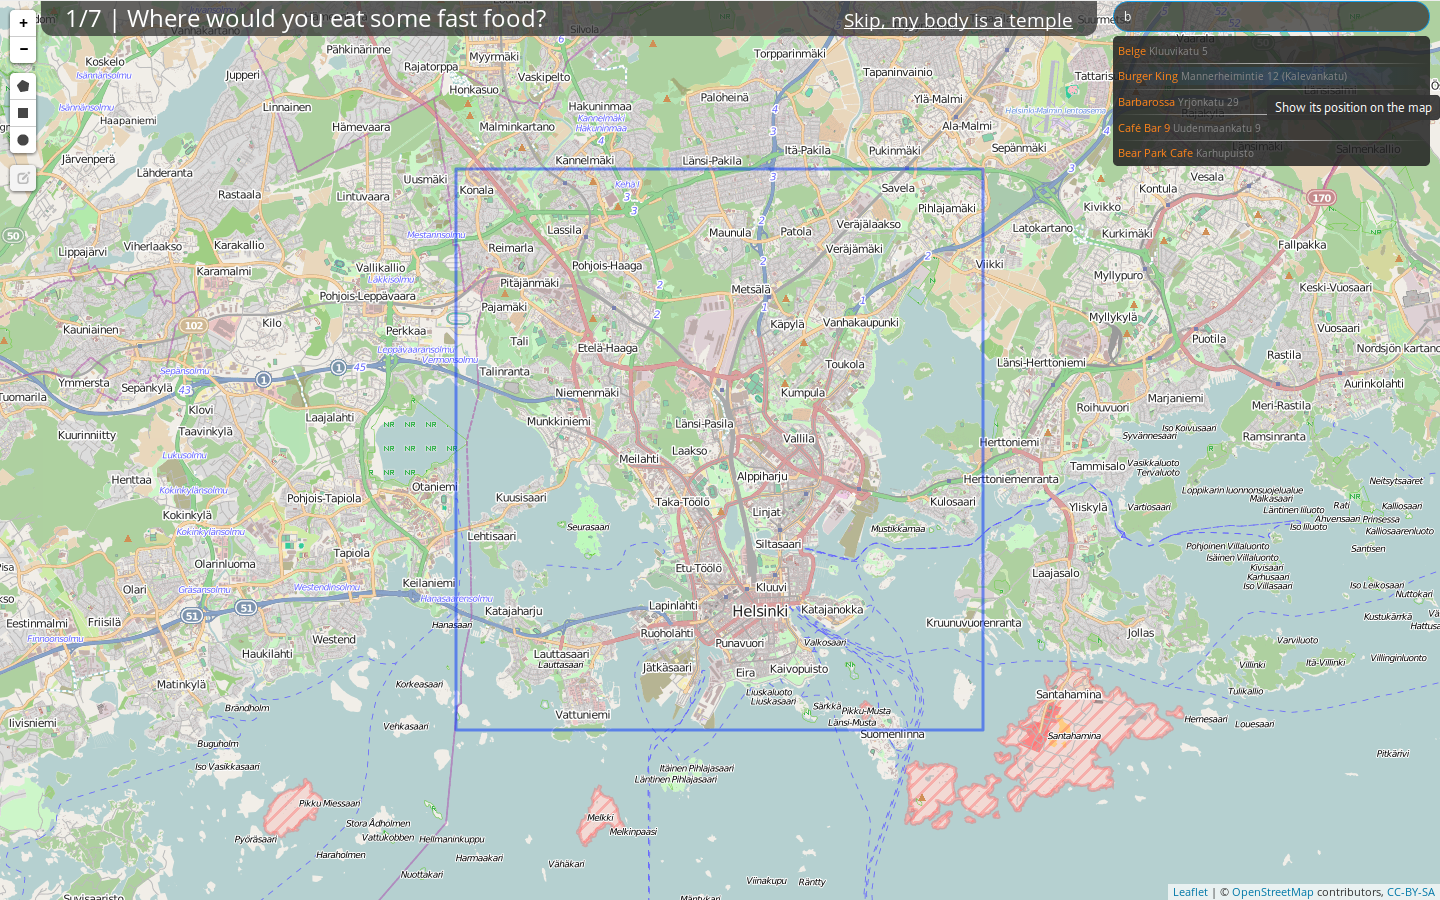
\includegraphics[width=\textwidth]{survey}
        \caption{The main screen of the survey.}
    \end{subfigure}

    \begin{subfigure}[b]{\textwidth}
        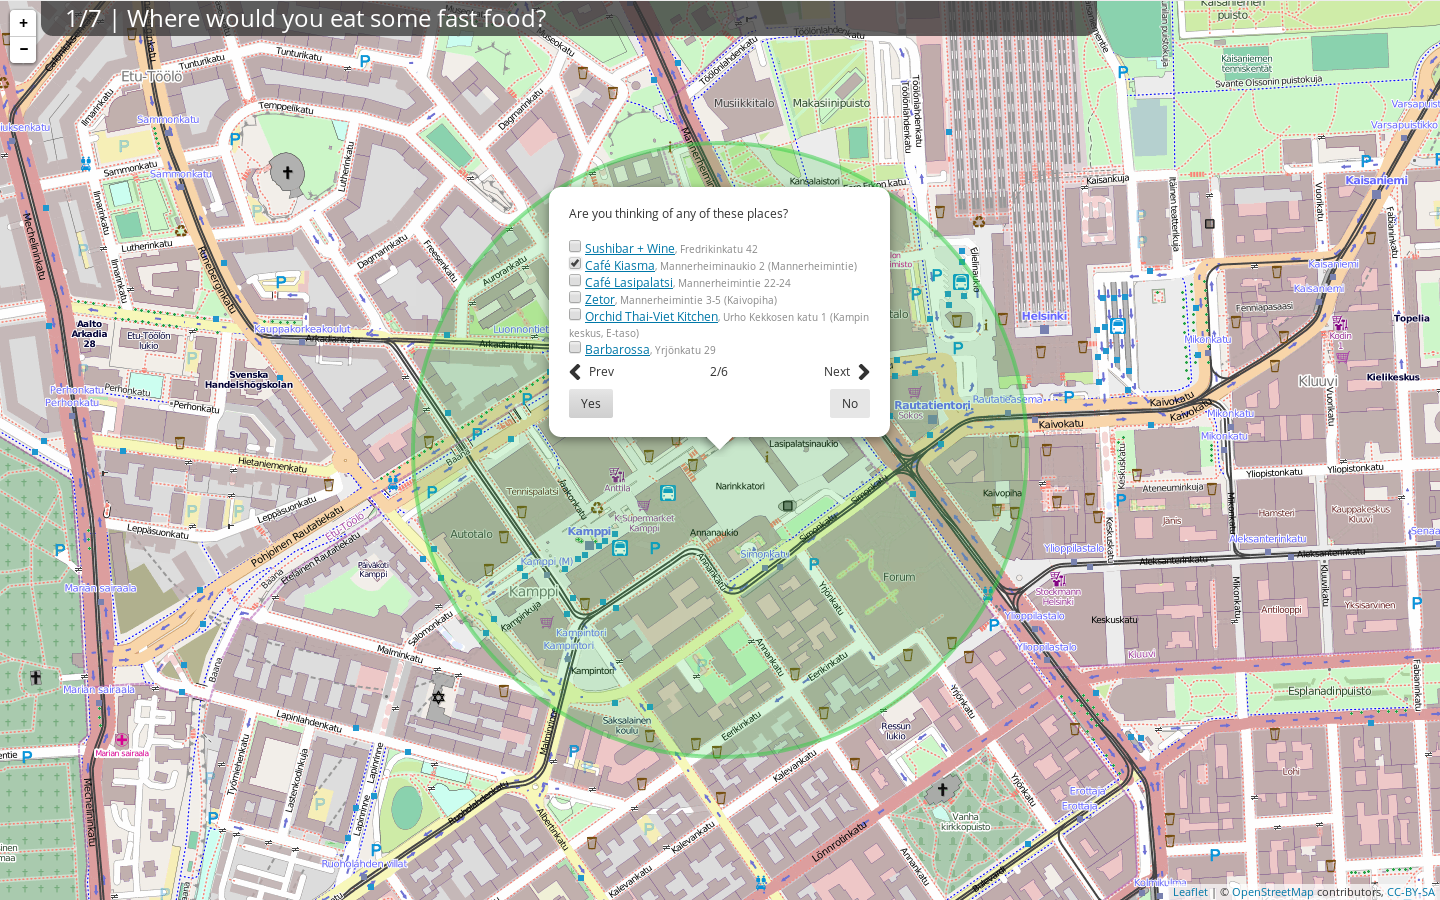
\includegraphics[width=\textwidth]{survey_venues}
        \caption{After an area have been drawn, the answer can be refined by
        choosing relevant venues from the dataset.}
    \end{subfigure}
    \caption{Website survey interface.\label{fig:survey}}
\end{figure}

number of answers, analysis of the results(?).

\begin{table}[ht]
    \centering
    \begin{tabularx}{\textwidth}{lXX}
        \toprule
	Name & Question label & Relevant categories \\
        \midrule
	\texttt{fastfood} & Where would you eat some fast food?                       & Food \\
	\texttt{romance}  & Where would you bring your date to a romantic restaurant? & Food \\
	\texttt{coffee}   & Where would you drink a cozy coffee?                      & Tea Room, Bistro, Café, Coffee Shop, Cafeteria \\
	\texttt{clothes}  & Where would you buy new fancy clothes?                    & Clothing Store, Department Store, Fabric Shop, Flea Market, Mall \\
	\texttt{party}    & Where would you hangout with your friends?                & Nightlife Spot \\
	\texttt{sport}    & Where would you go to run in nature?                      &  Outdoors \& Recreation \\
	\texttt{culture}  & Where would you enjoy some cultural attractions?          & Art Gallery, Comedy Club, Concert Hall, Country Dance Club, Historic Site, Museum, Movie Theater, Music Venue, Outdoor Sculpture, Performing Arts Venue, Public Art, Street Art \\
        \bottomrule
    \end{tabularx}
    \caption[Question list]{The seven questions asked to gather human
    input.\label{tab:questions}}
\end{table}

\section{Exploration}

While collecting this data, it was helpful to explore them, in order to
discover feature that could characterize places and help cluster them into
similar group.

\subsection{Time}

The time at which check-ins occur is undoubtedly a important variable. For
instance, \textcite{UrbanStory12} performed topic modelling from the text of
check-in tweets and showed that various topics exhibit daily or weekly
patterns. Likewise, \textcite{TimeCluster13} clustered cells of a rectangular
grid according to their repartition of check-ins over categories and time of
day.

Thus we first looked at when check-ins are performed, and how it differed from
city to city \autoref{fig:time_checkin}. Then we adopted a venue-centric view
and clustered locations according to which time they are active
\autoref{fig:day_cluster}, which also depend of the city
\autoref{fig:time_cluster_size}.

\begin{figure}[hbt]
    \begin{subfigure}[b]{\textwidth}
    \centering
    \iftoggle{EXTERNALPGF}{%
        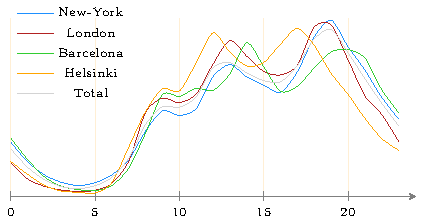
\includegraphics[width=\textwidth]{daily_checkin}
    }{%
        \begin{tikzpicture}
	\begin{axis}[xmin=0, xmax=24,
            unit vector ratio*=1 1.2,
	    axis y line=none,
            ymin=0, ymax=8.8,
            % title={Hourly check-ins frequency through the day},
            % xlabel={hour},
            % ylabel={percentage},
            legend style={at={(0.0,0.8)},anchor=west,draw=none,fill=none},
            grid=major
		]
\addplot[DodgerBlue,thin, smooth]table [x={time}, y={freq}] {newyork_day.dat};
\addlegendentry{New-York}
\addplot[FireBrick,thin, smooth]table [x={time}, y={freq}] {london_day.dat};
\addlegendentry{London}
\addplot[LimeGreen,thin, smooth]table [x={time}, y={freq}] {barcelona_day.dat};
\addlegendentry{Barcelona}
\addplot[Orange,thin, smooth]table [x={time}, y={freq}] {helsinki_day.dat};
\addlegendentry{Helsinki}
\addplot[LightGray,thin, smooth]table [x={time}, y={freq}] {global_day.dat};
\addlegendentry{Total}
\end{axis}
\end{tikzpicture}

    }
    \caption[Pattern of check-in during the day]{Generally, the activity is at
    its lowest around 5 a.m.\ and during the day, there are three peaks: one
when people go to work in the morning, one in the middle of the day and the
last one at the end of the evening. Yet, depending of the city, these peaks do
not happen at the same time, nor with the same intensity.
\label{fig:daily_checkin}}
    \end{subfigure}

    \begin{subfigure}[b]{\textwidth}
    \centering
    \iftoggle{EXTERNALPGF}{%
        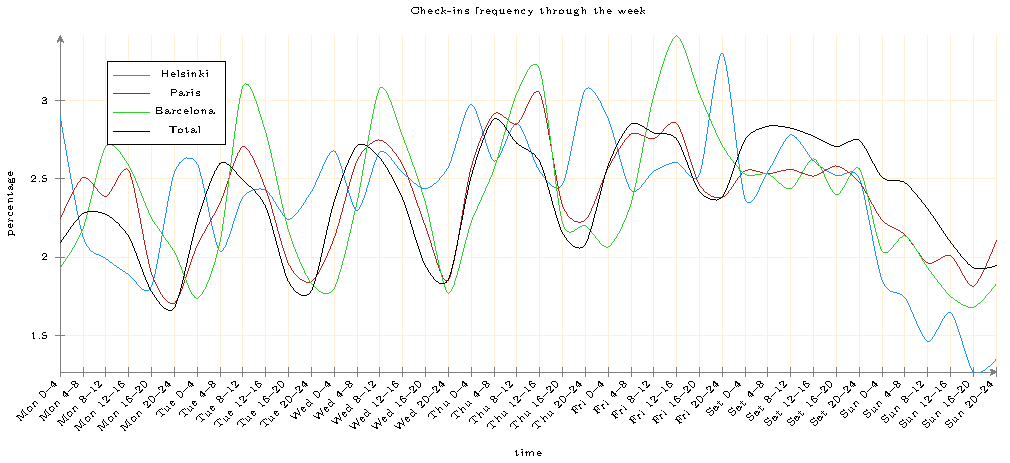
\includegraphics[width=\textwidth]{weekly_checkin}
    }{%
        %Mon 0--4, % Mon 4--8, Mon 8--12, % Mon 12--16, Mon 16--20, % Mon 20--24, Tue 0--4, % Tue 4--8, Tue 8--12, % Tue 12--16, Tue 16--20, % Tue 20--24, Wed 0--4, % Wed 4--8, Wed 8--12, % Wed 12--16, Wed 16--20, % Wed 20--24, Thu 0--4, % Thu 4--8, Thu 8--12, % Thu 12--16, Thu 16--20, % Thu 20--24, Fri 0--4, % Fri 4--8, Fri 8--12, % Fri 12--16, Fri 16--20, % Fri 20--24, Sat 0--4, % Sat 4--8, Sat 8--12, % Sat 12--16, Sat 16--20, % Sat 20--24, Sun 0--4, % Sun 4--8, Sun 8--12, % Sun 12--16, Sun 16--20, % Sun 20--24
\begin{tikzpicture}
    \begin{axis}[x={11},
            % title={Check-ins frequency through the week},
            % xlabel={time},
            % ylabel={percentage},
		    ymax=3.4,axis y line=none,
            legend
	    style={at={(0.76,0.00)},anchor=south,draw=none,fill=none,font=\Large,cells={line width=2pt}},
            x tick label style={rotate=45,anchor=east,font=\large},
            grid=major,
	    major grid style={line width=0.03pt, PapayaWhip},
	    xticklabels={%
		    Mon 0--4,,
		    % Mon 4--8,
		    Mon 8--12,,
		    % Mon 12--16,
		    Mon 16--20,,
		    % Mon 20--24,
		    Tue 0--4,,
		    % Tue 4--8,
		    Tue 8--12,,
		    % Tue 12--16,
		    Tue 16--20,,
		    % Tue 20--24,
		    Wed 0--4,,
		    % Wed 4--8,
		    Wed 8--12,,
		    % Wed 12--16,
		    Wed 16--20,,
		    % Wed 20--24,
		    Thu 0--4,,
		    % Thu 4--8,
		    Thu 8--12,,
		    % Thu 12--16,
		    Thu 16--20,,
		    % Thu 20--24,
		    Fri 0--4,,
		    % Fri 4--8,
		    Fri 8--12,,
		    % Fri 12--16,
		    Fri 16--20,,
		    % Fri 20--24,
		    Sat 0--4,,
		    % Sat 4--8,
		    Sat 8--12,,
		    % Sat 12--16,
		    Sat 16--20,,
		    % Sat 20--24,
		    Sun 0--4,,
		    % Sun 4--8,
		    Sun 8--12,,
		    % Sun 12--16,
		    Sun 16--20,,
		    % Sun 20--24
	    },
            xtick={0,...,41},
        ]
\addplot[DodgerBlue, smooth]table [x={time}, y={freq}] {newyork_week.dat};
\addlegendentry{New-York}
\addplot[FireBrick, smooth]table [x={time}, y={freq}] {london_week.dat};
\addlegendentry{London}
\addplot[LimeGreen, smooth]table [x={time}, y={freq}] {barcelona_week.dat};
\addlegendentry{Barcelona}
\addplot[Orange, smooth]table [x={time}, y={freq}] {helsinki_week.dat};
\addlegendentry{Helsinki}
\addplot[LightGray, smooth]table [x={time}, y={freq}] {global_week.dat};
\addlegendentry{Total}
% \addplot[DodgerBlue, smooth]table [x={time}, y={freq}] {helsinki_week.dat};
% \addlegendentry{Helsinki}
% \addplot[FireBrick, smooth]table [x={time}, y={freq}] {paris_week.dat};
% \addlegendentry{Paris}
% \addplot[LimeGreen, smooth]table [x={time}, y={freq}] {barcelona_week.dat};
% \addlegendentry{Barcelona}
% \addplot[Black, smooth]table [x={time}, y={freq}] {global_week.dat};
% \addlegendentry{Total}
\end{axis}
\end{tikzpicture}

    }
    \caption[Pattern of check-in during the week]{During the week, patterns
        are less clear.  \label{fig:weekly_checkin}}
    \end{subfigure}
    \caption{Check-ins temporal pattern.\label{fig:time_checkin}}
\end{figure}

\begin{figure}[hbt]
    \begin{subfigure}[b]{\textwidth}
    \centering
    \iftoggle{EXTERNALPGF}{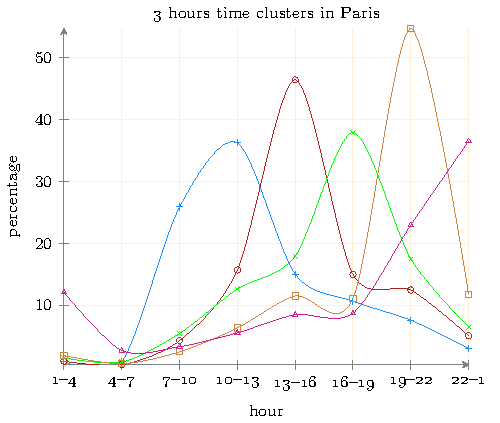
\includegraphics[width=\textwidth]{day_cluster_3h}}{\begin{tikzpicture}
	\begin{axis}[%
            title={3 hours time clusters in Paris},
            xlabel={hour},
            ylabel={percentage},
            % legend style={at={(0.05,0.8)},anchor=west},
            grid=major,
            xticklabels={,1--4, 4--7, 7--10, 10--13, 13--16, 16--19, 19--22, 22--1},
		]
\addplot[DodgerBlue , thin, smooth, mark size={1.5pt}, mark=+ ]table [x index=0, y index=1] {paris_cluster_day_3h.dat};
\addplot[FireBrick  , thin, smooth, mark size={1.5pt}, mark=o ]table      [x index=0, y index=2] {paris_cluster_day_3h.dat};
\addplot[Lime       , thin, smooth, mark size={1.5pt}, mark=x ]table [x index=0, y index=3] {paris_cluster_day_3h.dat};
\addplot[Peru       , thin, smooth, mark size={1.5pt}, mark=square ]table [x index=0, y index=4] {paris_cluster_day_3h.dat};
\addplot[VioletRed  , thin, smooth, mark size={1.5pt}, mark=triangle      ]table [x index=0, y index=5] {paris_cluster_day_3h.dat};
\end{axis}
\end{tikzpicture}


}
    \end{subfigure}

    \begin{subfigure}[b]{\textwidth}
    \centering
    \iftoggle{EXTERNALPGF}{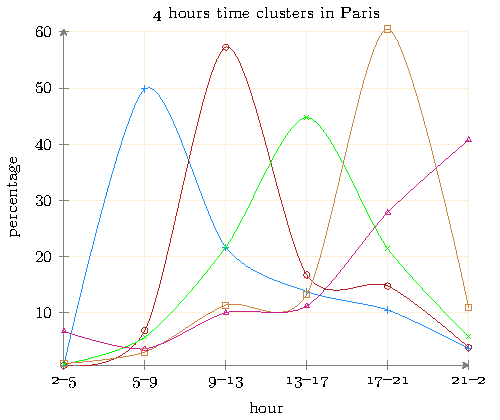
\includegraphics[width=\textwidth]{day_cluster_4h}}{\begin{tikzpicture}
	\begin{axis}[%
            title={4 hours time clusters in Paris},
            xlabel={hour},
            ylabel={percentage},
            % legend style={at={(0.05,0.8)},anchor=west},
            grid=major,
            xticklabels={,2--5,5--9,9--13,13--17,17--21,21--2}
		]
\addplot[DodgerBlue , thin, smooth, mark size={1.5pt}, mark=+ ]table [x index=0, y index=1] {paris_cluster_day_4h.dat};
\addplot[FireBrick  , thin, smooth, mark size={1.5pt}, mark=o ]table      [x index=0, y index=2] {paris_cluster_day_4h.dat};
\addplot[Lime       , thin, smooth, mark size={1.5pt}, mark=x ]table [x index=0, y index=3] {paris_cluster_day_4h.dat};
\addplot[Peru       , thin, smooth, mark size={1.5pt}, mark=square ]table [x index=0, y index=4] {paris_cluster_day_4h.dat};
\addplot[VioletRed  , thin, smooth, mark size={1.5pt}, mark=triangle      ]table [x index=0, y index=5] {paris_cluster_day_4h.dat};
\end{axis}
\end{tikzpicture}

}
    \end{subfigure}
    \caption[Venues clustered by time of check-ins]{Venues clustered by time
    of check-ins. \label{fig:day_cluster}}
\end{figure}

\newgeometry{left=0.3cm,right=0.3cm,bottom=0.1cm,top=0.1cm}
\begin{center}
\begin{figure}[hbt]
    \begin{subfigure}[b]{0.4\textwidth}
    \centering
    \iftoggle{EXTERNALPGF}{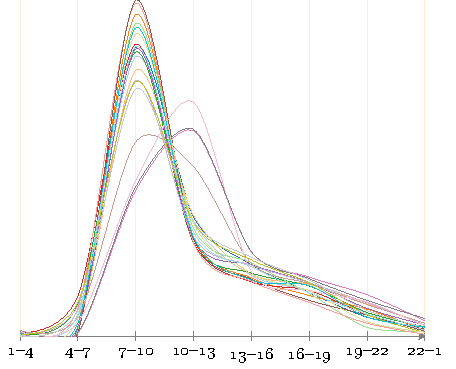
\includegraphics[height=0.18\textheight]{cluster_day_3h_cl1}}{\begin{tikzpicture}
	\begin{axis}[%
			axis y line=none,
            % title={3 hours Cluster 1 in all cities},
            % xlabel={hour},
            % ylabel={percentage},
            grid=major,
            xticklabels={,1--4, 4--7, 7--10, 10--13, 13--16, 16--19, 19--22, 22--1},
		]
\addplot[ck1, thin, smooth] table[x index=0, y index=1] {amsterdam_cluster_day_3h.dat};
\addplot[ck2, thin, smooth,] table[x index=0, y index=1]{atlanta_cluster_day_3h.dat};
\addplot[ck3, thin, smooth,] table[x index=0, y index=1]{barcelona_cluster_day_3h.dat};
\addplot[ck4, thin, smooth,] table[x index=0, y index=1]{berlin_cluster_day_3h.dat};
\addplot[ck5, thin, smooth,] table[x index=0, y index=1]{chicago_cluster_day_3h.dat};
\addplot[ck6, thin, smooth,] table[x index=0, y index=1]{helsinki_cluster_day_3h.dat};
\addplot[ck7, thin, smooth,] table[x index=0, y index=1]{houston_cluster_day_3h.dat};
\addplot[ck8, thin, smooth,] table[x index=0, y index=1]{indianapolis_cluster_day_3h.dat};
\addplot[ck9, thin, smooth,] table[x index=0, y index=1]{london_cluster_day_3h.dat};
\addplot[ck10, thin, smooth,] table[x index=0, y index=1]{losangeles_cluster_day_3h.dat};
\addplot[ck11, thin, smooth,] table[x index=0, y index=1]{moscow_cluster_day_3h.dat};
\addplot[ck12, thin, smooth,] table[x index=0, y index=1]{newyork_cluster_day_3h.dat};
\addplot[ck13, thin, smooth,] table[x index=0, y index=1]{paris_cluster_day_3h.dat};
\addplot[ck14, thin, smooth,] table[x index=0, y index=1]{prague_cluster_day_3h.dat};
\addplot[ck15, thin, smooth,] table[x index=0, y index=1]{rome_cluster_day_3h.dat};
\addplot[ck16, thin, smooth,] table[x index=0, y index=1]{sanfrancisco_cluster_day_3h.dat};
\addplot[ck17, thin, smooth,] table[x index=0, y index=1]{seattle_cluster_day_3h.dat};
\addplot[ck18, thin, smooth,] table[x index=0, y index=1]{stlouis_cluster_day_3h.dat};
\addplot[ck19, thin, smooth,] table[x index=0, y index=1]{stockholm_cluster_day_3h.dat};
\addplot[ck20, thin, smooth,] table[x index=0, y index=1]{washington_cluster_day_3h.dat};
\end{axis}
\end{tikzpicture}
}
    \end{subfigure}~
    \begin{subfigure}[b]{0.4\textwidth}
    \centering
    \iftoggle{EXTERNALPGF}{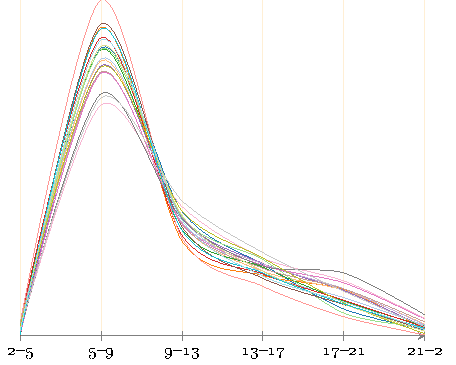
\includegraphics[height=0.18\textheight]{cluster_day_4h_cl1}}{\begin{tikzpicture}
	\begin{axis}[%
            title={ 4 hours Cluster 1 in all cities},
            xlabel={hour},
            ylabel={percentage},
            grid=major,
            xticklabels={,2--5,5--9,9--13,13--17,17--21,21--2}
		]
\addplot[ck1, thin, smooth] table[x index=0, y index=1] {amsterdam_cluster_day_4h.dat};
\addplot[ck2, thin, smooth,] table[x index=0, y index=1]{atlanta_cluster_day_4h.dat};
\addplot[ck3, thin, smooth,] table[x index=0, y index=1]{barcelona_cluster_day_4h.dat};
\addplot[ck4, thin, smooth,] table[x index=0, y index=1]{berlin_cluster_day_4h.dat};
\addplot[ck5, thin, smooth,] table[x index=0, y index=1]{chicago_cluster_day_4h.dat};
\addplot[ck6, thin, smooth,] table[x index=0, y index=1]{helsinki_cluster_day_4h.dat};
\addplot[ck7, thin, smooth,] table[x index=0, y index=1]{houston_cluster_day_4h.dat};
\addplot[ck8, thin, smooth,] table[x index=0, y index=1]{indianapolis_cluster_day_4h.dat};
\addplot[ck9, thin, smooth,] table[x index=0, y index=1]{london_cluster_day_4h.dat};
\addplot[ck10, thin, smooth,] table[x index=0, y index=1]{losangeles_cluster_day_4h.dat};
\addplot[ck11, thin, smooth,] table[x index=0, y index=1]{moscow_cluster_day_4h.dat};
\addplot[ck12, thin, smooth,] table[x index=0, y index=1]{newyork_cluster_day_4h.dat};
\addplot[ck13, thin, smooth,] table[x index=0, y index=1]{paris_cluster_day_4h.dat};
\addplot[ck14, thin, smooth,] table[x index=0, y index=1]{prague_cluster_day_4h.dat};
\addplot[ck15, thin, smooth,] table[x index=0, y index=1]{rome_cluster_day_4h.dat};
\addplot[ck16, thin, smooth,] table[x index=0, y index=1]{sanfrancisco_cluster_day_4h.dat};
\addplot[ck17, thin, smooth,] table[x index=0, y index=1]{seattle_cluster_day_4h.dat};
\addplot[ck18, thin, smooth,] table[x index=0, y index=1]{stlouis_cluster_day_4h.dat};
\addplot[ck19, thin, smooth,] table[x index=0, y index=1]{stockholm_cluster_day_4h.dat};
\addplot[ck20, thin, smooth,] table[x index=0, y index=1]{washington_cluster_day_4h.dat};
\end{axis}
\end{tikzpicture}
}
    \end{subfigure}

    \begin{subfigure}[b]{0.4\textwidth}
    \centering
    \iftoggle{EXTERNALPGF}{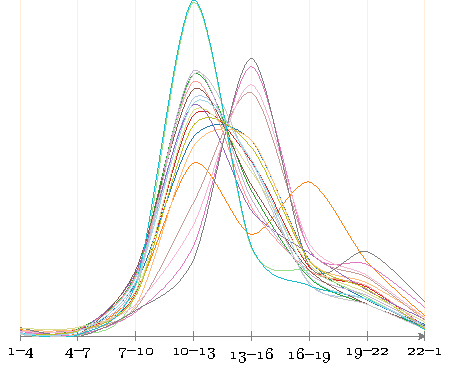
\includegraphics[height=0.18\textheight]{cluster_day_3h_cl2}}{\begin{tikzpicture}
	\begin{axis}[%
			axis y line=none,
            % title={3 hours Cluster 2 in all cities},
            % xlabel={hour},
            % ylabel={percentage},
            grid=major,
            xticklabels={,1--4, 4--7, 7--10, 10--13, 13--16, 16--19, 19--22, 22--1},
		]
\addplot[ck1, thin, smooth] table[x index=0, y index=2] {amsterdam_cluster_day_3h.dat};
\addplot[ck2, thin, smooth,] table[x index=0, y index=2]{atlanta_cluster_day_3h.dat};
\addplot[ck3, thin, smooth,] table[x index=0, y index=2]{barcelona_cluster_day_3h.dat};
\addplot[ck4, thin, smooth,] table[x index=0, y index=2]{berlin_cluster_day_3h.dat};
\addplot[ck5, thin, smooth,] table[x index=0, y index=2]{chicago_cluster_day_3h.dat};
\addplot[ck6, thin, smooth,] table[x index=0, y index=2]{helsinki_cluster_day_3h.dat};
\addplot[ck7, thin, smooth,] table[x index=0, y index=2]{houston_cluster_day_3h.dat};
\addplot[ck8, thin, smooth,] table[x index=0, y index=2]{indianapolis_cluster_day_3h.dat};
\addplot[ck9, thin, smooth,] table[x index=0, y index=2]{london_cluster_day_3h.dat};
\addplot[ck10, thin, smooth,] table[x index=0, y index=2]{losangeles_cluster_day_3h.dat};
\addplot[ck11, thin, smooth,] table[x index=0, y index=2]{moscow_cluster_day_3h.dat};
\addplot[ck12, thin, smooth,] table[x index=0, y index=2]{newyork_cluster_day_3h.dat};
\addplot[ck13, thin, smooth,] table[x index=0, y index=2]{paris_cluster_day_3h.dat};
\addplot[ck14, thin, smooth,] table[x index=0, y index=2]{prague_cluster_day_3h.dat};
\addplot[ck15, thin, smooth,] table[x index=0, y index=2]{rome_cluster_day_3h.dat};
\addplot[ck16, thin, smooth,] table[x index=0, y index=2]{sanfrancisco_cluster_day_3h.dat};
\addplot[ck17, thin, smooth,] table[x index=0, y index=2]{seattle_cluster_day_3h.dat};
\addplot[ck18, thin, smooth,] table[x index=0, y index=2]{stlouis_cluster_day_3h.dat};
\addplot[ck19, thin, smooth,] table[x index=0, y index=2]{stockholm_cluster_day_3h.dat};
\addplot[ck20, thin, smooth,] table[x index=0, y index=2]{washington_cluster_day_3h.dat};
\end{axis}
\end{tikzpicture}
}
    \end{subfigure}~
    \begin{subfigure}[b]{0.4\textwidth}
    \centering
    \iftoggle{EXTERNALPGF}{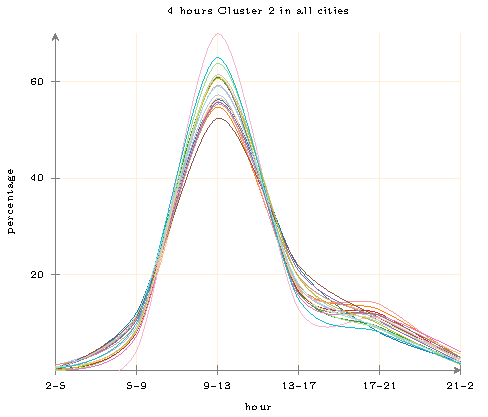
\includegraphics[height=0.18\textheight]{cluster_day_4h_cl2}}{\begin{tikzpicture}
	\begin{axis}[%
            title={ 4 hours Cluster 2 in all cities},
            xlabel={hour},
            ylabel={percentage},
            grid=major,
            xticklabels={,2--5,5--9,9--13,13--17,17--21,21--2}
		]
\addplot[ck1, thin, smooth] table[x index=0, y index=2] {amsterdam_cluster_day_4h.dat};
\addplot[ck2, thin, smooth,] table[x index=0, y index=2]{atlanta_cluster_day_4h.dat};
\addplot[ck3, thin, smooth,] table[x index=0, y index=2]{barcelona_cluster_day_4h.dat};
\addplot[ck4, thin, smooth,] table[x index=0, y index=2]{berlin_cluster_day_4h.dat};
\addplot[ck5, thin, smooth,] table[x index=0, y index=2]{chicago_cluster_day_4h.dat};
\addplot[ck6, thin, smooth,] table[x index=0, y index=2]{helsinki_cluster_day_4h.dat};
\addplot[ck7, thin, smooth,] table[x index=0, y index=2]{houston_cluster_day_4h.dat};
\addplot[ck8, thin, smooth,] table[x index=0, y index=2]{indianapolis_cluster_day_4h.dat};
\addplot[ck9, thin, smooth,] table[x index=0, y index=2]{london_cluster_day_4h.dat};
\addplot[ck10, thin, smooth,] table[x index=0, y index=2]{losangeles_cluster_day_4h.dat};
\addplot[ck11, thin, smooth,] table[x index=0, y index=2]{moscow_cluster_day_4h.dat};
\addplot[ck12, thin, smooth,] table[x index=0, y index=2]{newyork_cluster_day_4h.dat};
\addplot[ck13, thin, smooth,] table[x index=0, y index=2]{paris_cluster_day_4h.dat};
\addplot[ck14, thin, smooth,] table[x index=0, y index=2]{prague_cluster_day_4h.dat};
\addplot[ck15, thin, smooth,] table[x index=0, y index=2]{rome_cluster_day_4h.dat};
\addplot[ck16, thin, smooth,] table[x index=0, y index=2]{sanfrancisco_cluster_day_4h.dat};
\addplot[ck17, thin, smooth,] table[x index=0, y index=2]{seattle_cluster_day_4h.dat};
\addplot[ck18, thin, smooth,] table[x index=0, y index=2]{stlouis_cluster_day_4h.dat};
\addplot[ck19, thin, smooth,] table[x index=0, y index=2]{stockholm_cluster_day_4h.dat};
\addplot[ck20, thin, smooth,] table[x index=0, y index=2]{washington_cluster_day_4h.dat};
\end{axis}
\end{tikzpicture}
}
    \end{subfigure}

    \begin{subfigure}[b]{0.4\textwidth}
    \centering
    \iftoggle{EXTERNALPGF}{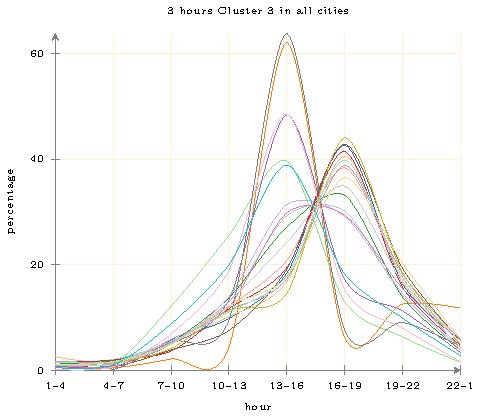
\includegraphics[height=0.18\textheight]{cluster_day_3h_cl3}}{\begin{tikzpicture}
	\begin{axis}[%
            title={3 hours Cluster 3 in all cities},
            xlabel={hour},
            ylabel={percentage},
            grid=major,
            xticklabels={,1--4, 4--7, 7--10, 10--13, 13--16, 16--19, 19--22, 22--1},
		]
\addplot[ck1, thin, smooth] table[x index=0, y index=3] {amsterdam_cluster_day_3h.dat};
\addplot[ck2, thin, smooth,] table[x index=0, y index=3]{atlanta_cluster_day_3h.dat};
\addplot[ck3, thin, smooth,] table[x index=0, y index=3]{barcelona_cluster_day_3h.dat};
\addplot[ck4, thin, smooth,] table[x index=0, y index=3]{berlin_cluster_day_3h.dat};
\addplot[ck5, thin, smooth,] table[x index=0, y index=3]{chicago_cluster_day_3h.dat};
\addplot[ck6, thin, smooth,] table[x index=0, y index=3]{helsinki_cluster_day_3h.dat};
\addplot[ck7, thin, smooth,] table[x index=0, y index=3]{houston_cluster_day_3h.dat};
\addplot[ck8, thin, smooth,] table[x index=0, y index=3]{indianapolis_cluster_day_3h.dat};
\addplot[ck9, thin, smooth,] table[x index=0, y index=3]{london_cluster_day_3h.dat};
\addplot[ck10, thin, smooth,] table[x index=0, y index=3]{losangeles_cluster_day_3h.dat};
\addplot[ck11, thin, smooth,] table[x index=0, y index=3]{moscow_cluster_day_3h.dat};
\addplot[ck12, thin, smooth,] table[x index=0, y index=3]{newyork_cluster_day_3h.dat};
\addplot[ck13, thin, smooth,] table[x index=0, y index=3]{paris_cluster_day_3h.dat};
\addplot[ck14, thin, smooth,] table[x index=0, y index=3]{prague_cluster_day_3h.dat};
\addplot[ck15, thin, smooth,] table[x index=0, y index=3]{rome_cluster_day_3h.dat};
\addplot[ck16, thin, smooth,] table[x index=0, y index=3]{sanfrancisco_cluster_day_3h.dat};
\addplot[ck17, thin, smooth,] table[x index=0, y index=3]{seattle_cluster_day_3h.dat};
\addplot[ck18, thin, smooth,] table[x index=0, y index=3]{stlouis_cluster_day_3h.dat};
\addplot[ck19, thin, smooth,] table[x index=0, y index=3]{stockholm_cluster_day_3h.dat};
\addplot[ck20, thin, smooth,] table[x index=0, y index=3]{washington_cluster_day_3h.dat};
\end{axis}
\end{tikzpicture}
}
    \end{subfigure}~
    \begin{subfigure}[b]{0.4\textwidth}
    \centering
    \iftoggle{EXTERNALPGF}{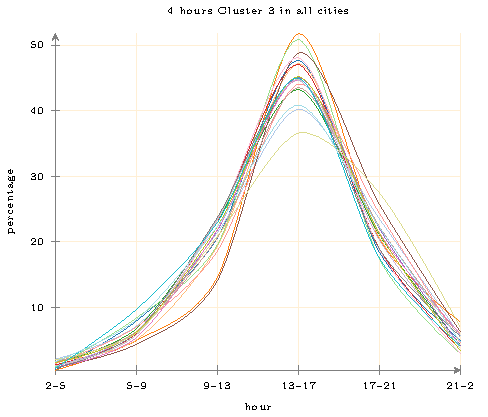
\includegraphics[height=0.18\textheight]{cluster_day_4h_cl3}}{\begin{tikzpicture}
	\begin{axis}[%
            title={ 4 hours Cluster 3 in all cities},
            xlabel={hour},
            ylabel={percentage},
            grid=major,
            xticklabels={,2--5,5--9,9--13,13--17,17--21,21--2}
		]
\addplot[ck1, thin, smooth] table[x index=0, y index=3] {amsterdam_cluster_day_4h.dat};
\addplot[ck2, thin, smooth,] table[x index=0, y index=3]{atlanta_cluster_day_4h.dat};
\addplot[ck3, thin, smooth,] table[x index=0, y index=3]{barcelona_cluster_day_4h.dat};
\addplot[ck4, thin, smooth,] table[x index=0, y index=3]{berlin_cluster_day_4h.dat};
\addplot[ck5, thin, smooth,] table[x index=0, y index=3]{chicago_cluster_day_4h.dat};
\addplot[ck6, thin, smooth,] table[x index=0, y index=3]{helsinki_cluster_day_4h.dat};
\addplot[ck7, thin, smooth,] table[x index=0, y index=3]{houston_cluster_day_4h.dat};
\addplot[ck8, thin, smooth,] table[x index=0, y index=3]{indianapolis_cluster_day_4h.dat};
\addplot[ck9, thin, smooth,] table[x index=0, y index=3]{london_cluster_day_4h.dat};
\addplot[ck10, thin, smooth,] table[x index=0, y index=3]{losangeles_cluster_day_4h.dat};
\addplot[ck11, thin, smooth,] table[x index=0, y index=3]{moscow_cluster_day_4h.dat};
\addplot[ck12, thin, smooth,] table[x index=0, y index=3]{newyork_cluster_day_4h.dat};
\addplot[ck13, thin, smooth,] table[x index=0, y index=3]{paris_cluster_day_4h.dat};
\addplot[ck14, thin, smooth,] table[x index=0, y index=3]{prague_cluster_day_4h.dat};
\addplot[ck15, thin, smooth,] table[x index=0, y index=3]{rome_cluster_day_4h.dat};
\addplot[ck16, thin, smooth,] table[x index=0, y index=3]{sanfrancisco_cluster_day_4h.dat};
\addplot[ck17, thin, smooth,] table[x index=0, y index=3]{seattle_cluster_day_4h.dat};
\addplot[ck18, thin, smooth,] table[x index=0, y index=3]{stlouis_cluster_day_4h.dat};
\addplot[ck19, thin, smooth,] table[x index=0, y index=3]{stockholm_cluster_day_4h.dat};
\addplot[ck20, thin, smooth,] table[x index=0, y index=3]{washington_cluster_day_4h.dat};
\end{axis}
\end{tikzpicture}
}
    \end{subfigure}

    \begin{subfigure}[b]{0.4\textwidth}
    \centering
    \iftoggle{EXTERNALPGF}{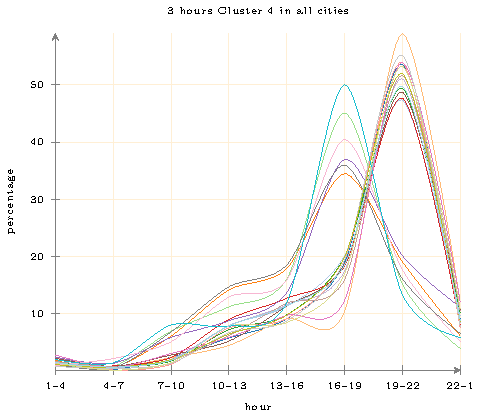
\includegraphics[height=0.18\textheight]{cluster_day_3h_cl4}}{\begin{tikzpicture}
	\begin{axis}[%
            title={3 hours Cluster 4 in all cities},
            xlabel={hour},
            ylabel={percentage},
            grid=major,
            xticklabels={,1--4, 4--7, 7--10, 10--13, 13--16, 16--19, 19--22, 22--1},
		]
\addplot[ck1, thin, smooth] table[x index=0, y index=4] {amsterdam_cluster_day_3h.dat};
\addplot[ck2, thin, smooth,] table[x index=0, y index=4]{atlanta_cluster_day_3h.dat};
\addplot[ck3, thin, smooth,] table[x index=0, y index=4]{barcelona_cluster_day_3h.dat};
\addplot[ck4, thin, smooth,] table[x index=0, y index=4]{berlin_cluster_day_3h.dat};
\addplot[ck5, thin, smooth,] table[x index=0, y index=4]{chicago_cluster_day_3h.dat};
\addplot[ck6, thin, smooth,] table[x index=0, y index=4]{helsinki_cluster_day_3h.dat};
\addplot[ck7, thin, smooth,] table[x index=0, y index=4]{houston_cluster_day_3h.dat};
\addplot[ck8, thin, smooth,] table[x index=0, y index=4]{indianapolis_cluster_day_3h.dat};
\addplot[ck9, thin, smooth,] table[x index=0, y index=4]{london_cluster_day_3h.dat};
\addplot[ck10, thin, smooth,] table[x index=0, y index=4]{losangeles_cluster_day_3h.dat};
\addplot[ck11, thin, smooth,] table[x index=0, y index=4]{moscow_cluster_day_3h.dat};
\addplot[ck12, thin, smooth,] table[x index=0, y index=4]{newyork_cluster_day_3h.dat};
\addplot[ck13, thin, smooth,] table[x index=0, y index=4]{paris_cluster_day_3h.dat};
\addplot[ck14, thin, smooth,] table[x index=0, y index=4]{prague_cluster_day_3h.dat};
\addplot[ck15, thin, smooth,] table[x index=0, y index=4]{rome_cluster_day_3h.dat};
\addplot[ck16, thin, smooth,] table[x index=0, y index=4]{sanfrancisco_cluster_day_3h.dat};
\addplot[ck17, thin, smooth,] table[x index=0, y index=4]{seattle_cluster_day_3h.dat};
\addplot[ck18, thin, smooth,] table[x index=0, y index=4]{stlouis_cluster_day_3h.dat};
\addplot[ck19, thin, smooth,] table[x index=0, y index=4]{stockholm_cluster_day_3h.dat};
\addplot[ck20, thin, smooth,] table[x index=0, y index=4]{washington_cluster_day_3h.dat};
\end{axis}
\end{tikzpicture}
}
    \end{subfigure}~
    \begin{subfigure}[b]{0.4\textwidth}
    \centering
    \iftoggle{EXTERNALPGF}{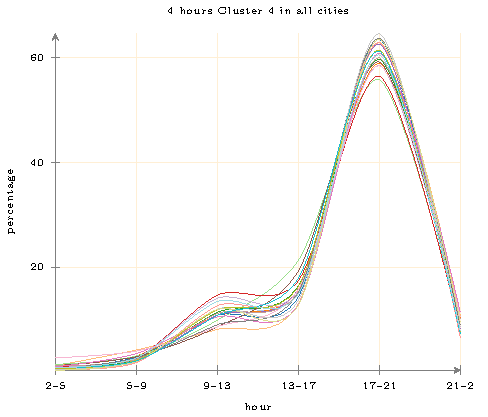
\includegraphics[height=0.18\textheight]{cluster_day_4h_cl4}}{\begin{tikzpicture}
	\begin{axis}[%
            title={ 4 hours Cluster 4 in all cities},
            xlabel={hour},
            ylabel={percentage},
            grid=major,
            xticklabels={,2--5,5--9,9--13,13--17,17--21,21--2}
		]
\addplot[ck1, thin, smooth] table[x index=0, y index=4] {amsterdam_cluster_day_4h.dat};
\addplot[ck2, thin, smooth,] table[x index=0, y index=4]{atlanta_cluster_day_4h.dat};
\addplot[ck3, thin, smooth,] table[x index=0, y index=4]{barcelona_cluster_day_4h.dat};
\addplot[ck4, thin, smooth,] table[x index=0, y index=4]{berlin_cluster_day_4h.dat};
\addplot[ck5, thin, smooth,] table[x index=0, y index=4]{chicago_cluster_day_4h.dat};
\addplot[ck6, thin, smooth,] table[x index=0, y index=4]{helsinki_cluster_day_4h.dat};
\addplot[ck7, thin, smooth,] table[x index=0, y index=4]{houston_cluster_day_4h.dat};
\addplot[ck8, thin, smooth,] table[x index=0, y index=4]{indianapolis_cluster_day_4h.dat};
\addplot[ck9, thin, smooth,] table[x index=0, y index=4]{london_cluster_day_4h.dat};
\addplot[ck10, thin, smooth,] table[x index=0, y index=4]{losangeles_cluster_day_4h.dat};
\addplot[ck11, thin, smooth,] table[x index=0, y index=4]{moscow_cluster_day_4h.dat};
\addplot[ck12, thin, smooth,] table[x index=0, y index=4]{newyork_cluster_day_4h.dat};
\addplot[ck13, thin, smooth,] table[x index=0, y index=4]{paris_cluster_day_4h.dat};
\addplot[ck14, thin, smooth,] table[x index=0, y index=4]{prague_cluster_day_4h.dat};
\addplot[ck15, thin, smooth,] table[x index=0, y index=4]{rome_cluster_day_4h.dat};
\addplot[ck16, thin, smooth,] table[x index=0, y index=4]{sanfrancisco_cluster_day_4h.dat};
\addplot[ck17, thin, smooth,] table[x index=0, y index=4]{seattle_cluster_day_4h.dat};
\addplot[ck18, thin, smooth,] table[x index=0, y index=4]{stlouis_cluster_day_4h.dat};
\addplot[ck19, thin, smooth,] table[x index=0, y index=4]{stockholm_cluster_day_4h.dat};
\addplot[ck20, thin, smooth,] table[x index=0, y index=4]{washington_cluster_day_4h.dat};
\end{axis}
\end{tikzpicture}
}
    \end{subfigure}

    \begin{subfigure}[b]{0.4\textwidth}
    \centering
    \iftoggle{EXTERNALPGF}{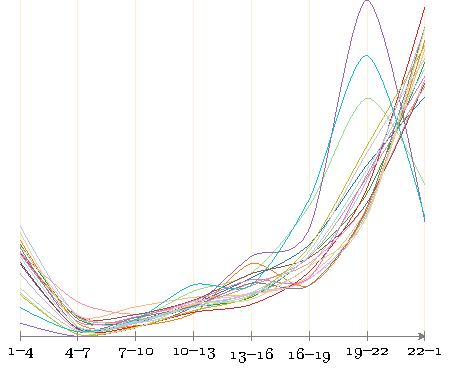
\includegraphics[height=0.18\textheight]{cluster_day_3h_cl5}}{\begin{tikzpicture}
	\begin{axis}[%
			axis y line=none,
            % title={3 hours Cluster 5 in all cities},
            % xlabel={hour},
            % ylabel={percentage},
            grid=major,
            xticklabels={,1--4, 4--7, 7--10, 10--13, 13--16, 16--19, 19--22, 22--1},
		]
\addplot[ck1, thin, smooth] table[x index=0, y index=5] {amsterdam_cluster_day_3h.dat};
\addplot[ck2, thin, smooth,] table[x index=0, y index=5]{atlanta_cluster_day_3h.dat};
\addplot[ck3, thin, smooth,] table[x index=0, y index=5]{barcelona_cluster_day_3h.dat};
\addplot[ck4, thin, smooth,] table[x index=0, y index=5]{berlin_cluster_day_3h.dat};
\addplot[ck5, thin, smooth,] table[x index=0, y index=5]{chicago_cluster_day_3h.dat};
\addplot[ck6, thin, smooth,] table[x index=0, y index=5]{helsinki_cluster_day_3h.dat};
\addplot[ck7, thin, smooth,] table[x index=0, y index=5]{houston_cluster_day_3h.dat};
\addplot[ck8, thin, smooth,] table[x index=0, y index=5]{indianapolis_cluster_day_3h.dat};
\addplot[ck9, thin, smooth,] table[x index=0, y index=5]{london_cluster_day_3h.dat};
\addplot[ck10, thin, smooth,] table[x index=0, y index=5]{losangeles_cluster_day_3h.dat};
\addplot[ck11, thin, smooth,] table[x index=0, y index=5]{moscow_cluster_day_3h.dat};
\addplot[ck12, thin, smooth,] table[x index=0, y index=5]{newyork_cluster_day_3h.dat};
\addplot[ck13, thin, smooth,] table[x index=0, y index=5]{paris_cluster_day_3h.dat};
\addplot[ck14, thin, smooth,] table[x index=0, y index=5]{prague_cluster_day_3h.dat};
\addplot[ck15, thin, smooth,] table[x index=0, y index=5]{rome_cluster_day_3h.dat};
\addplot[ck16, thin, smooth,] table[x index=0, y index=5]{sanfrancisco_cluster_day_3h.dat};
\addplot[ck17, thin, smooth,] table[x index=0, y index=5]{seattle_cluster_day_3h.dat};
\addplot[ck18, thin, smooth,] table[x index=0, y index=5]{stlouis_cluster_day_3h.dat};
\addplot[ck19, thin, smooth,] table[x index=0, y index=5]{stockholm_cluster_day_3h.dat};
\addplot[ck20, thin, smooth,] table[x index=0, y index=5]{washington_cluster_day_3h.dat};
\end{axis}
\end{tikzpicture}
}
    \end{subfigure}~
    \begin{subfigure}[b]{0.4\textwidth}
    \centering
    \iftoggle{EXTERNALPGF}{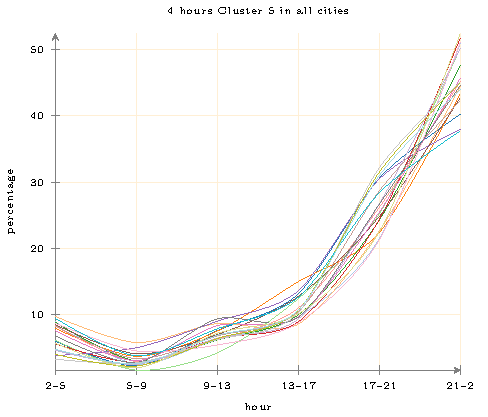
\includegraphics[height=0.18\textheight]{cluster_day_4h_cl5}}{\begin{tikzpicture}
	\begin{axis}[%
			axis y line=none,
            grid=major,
            xticklabels={,2--5,5--9,9--13,13--17,17--21,21--2}
		]
\addplot[ck1, thin, smooth] table[x index=0, y index=5] {amsterdam_cluster_day_4h.dat};
\addplot[ck2, thin, smooth,] table[x index=0, y index=5]{atlanta_cluster_day_4h.dat};
\addplot[ck3, thin, smooth,] table[x index=0, y index=5]{barcelona_cluster_day_4h.dat};
\addplot[ck4, thin, smooth,] table[x index=0, y index=5]{berlin_cluster_day_4h.dat};
\addplot[ck5, thin, smooth,] table[x index=0, y index=5]{chicago_cluster_day_4h.dat};
\addplot[ck6, thin, smooth,] table[x index=0, y index=5]{helsinki_cluster_day_4h.dat};
\addplot[ck7, thin, smooth,] table[x index=0, y index=5]{houston_cluster_day_4h.dat};
\addplot[ck8, thin, smooth,] table[x index=0, y index=5]{indianapolis_cluster_day_4h.dat};
\addplot[ck9, thin, smooth,] table[x index=0, y index=5]{london_cluster_day_4h.dat};
\addplot[ck10, thin, smooth,] table[x index=0, y index=5]{losangeles_cluster_day_4h.dat};
\addplot[ck11, thin, smooth,] table[x index=0, y index=5]{moscow_cluster_day_4h.dat};
\addplot[ck12, thin, smooth,] table[x index=0, y index=5]{newyork_cluster_day_4h.dat};
\addplot[ck13, thin, smooth,] table[x index=0, y index=5]{paris_cluster_day_4h.dat};
\addplot[ck14, thin, smooth,] table[x index=0, y index=5]{prague_cluster_day_4h.dat};
\addplot[ck15, thin, smooth,] table[x index=0, y index=5]{rome_cluster_day_4h.dat};
\addplot[ck16, thin, smooth,] table[x index=0, y index=5]{sanfrancisco_cluster_day_4h.dat};
\addplot[ck17, thin, smooth,] table[x index=0, y index=5]{seattle_cluster_day_4h.dat};
\addplot[ck18, thin, smooth,] table[x index=0, y index=5]{stlouis_cluster_day_4h.dat};
\addplot[ck19, thin, smooth,] table[x index=0, y index=5]{stockholm_cluster_day_4h.dat};
\addplot[ck20, thin, smooth,] table[x index=0, y index=5]{washington_cluster_day_4h.dat};
\end{axis}
\end{tikzpicture}
}
    \end{subfigure}
    \caption[Venues cluster by time among all the cities]{4 hours time
    clusters are the same among all cities, whereas it is not the case for 3
hours clusters. \label{fig:time_cluster_size}}
\end{figure}
\end{center}
\restoregeometry

\subsection{Space}

\begin{figure}[hbtp]
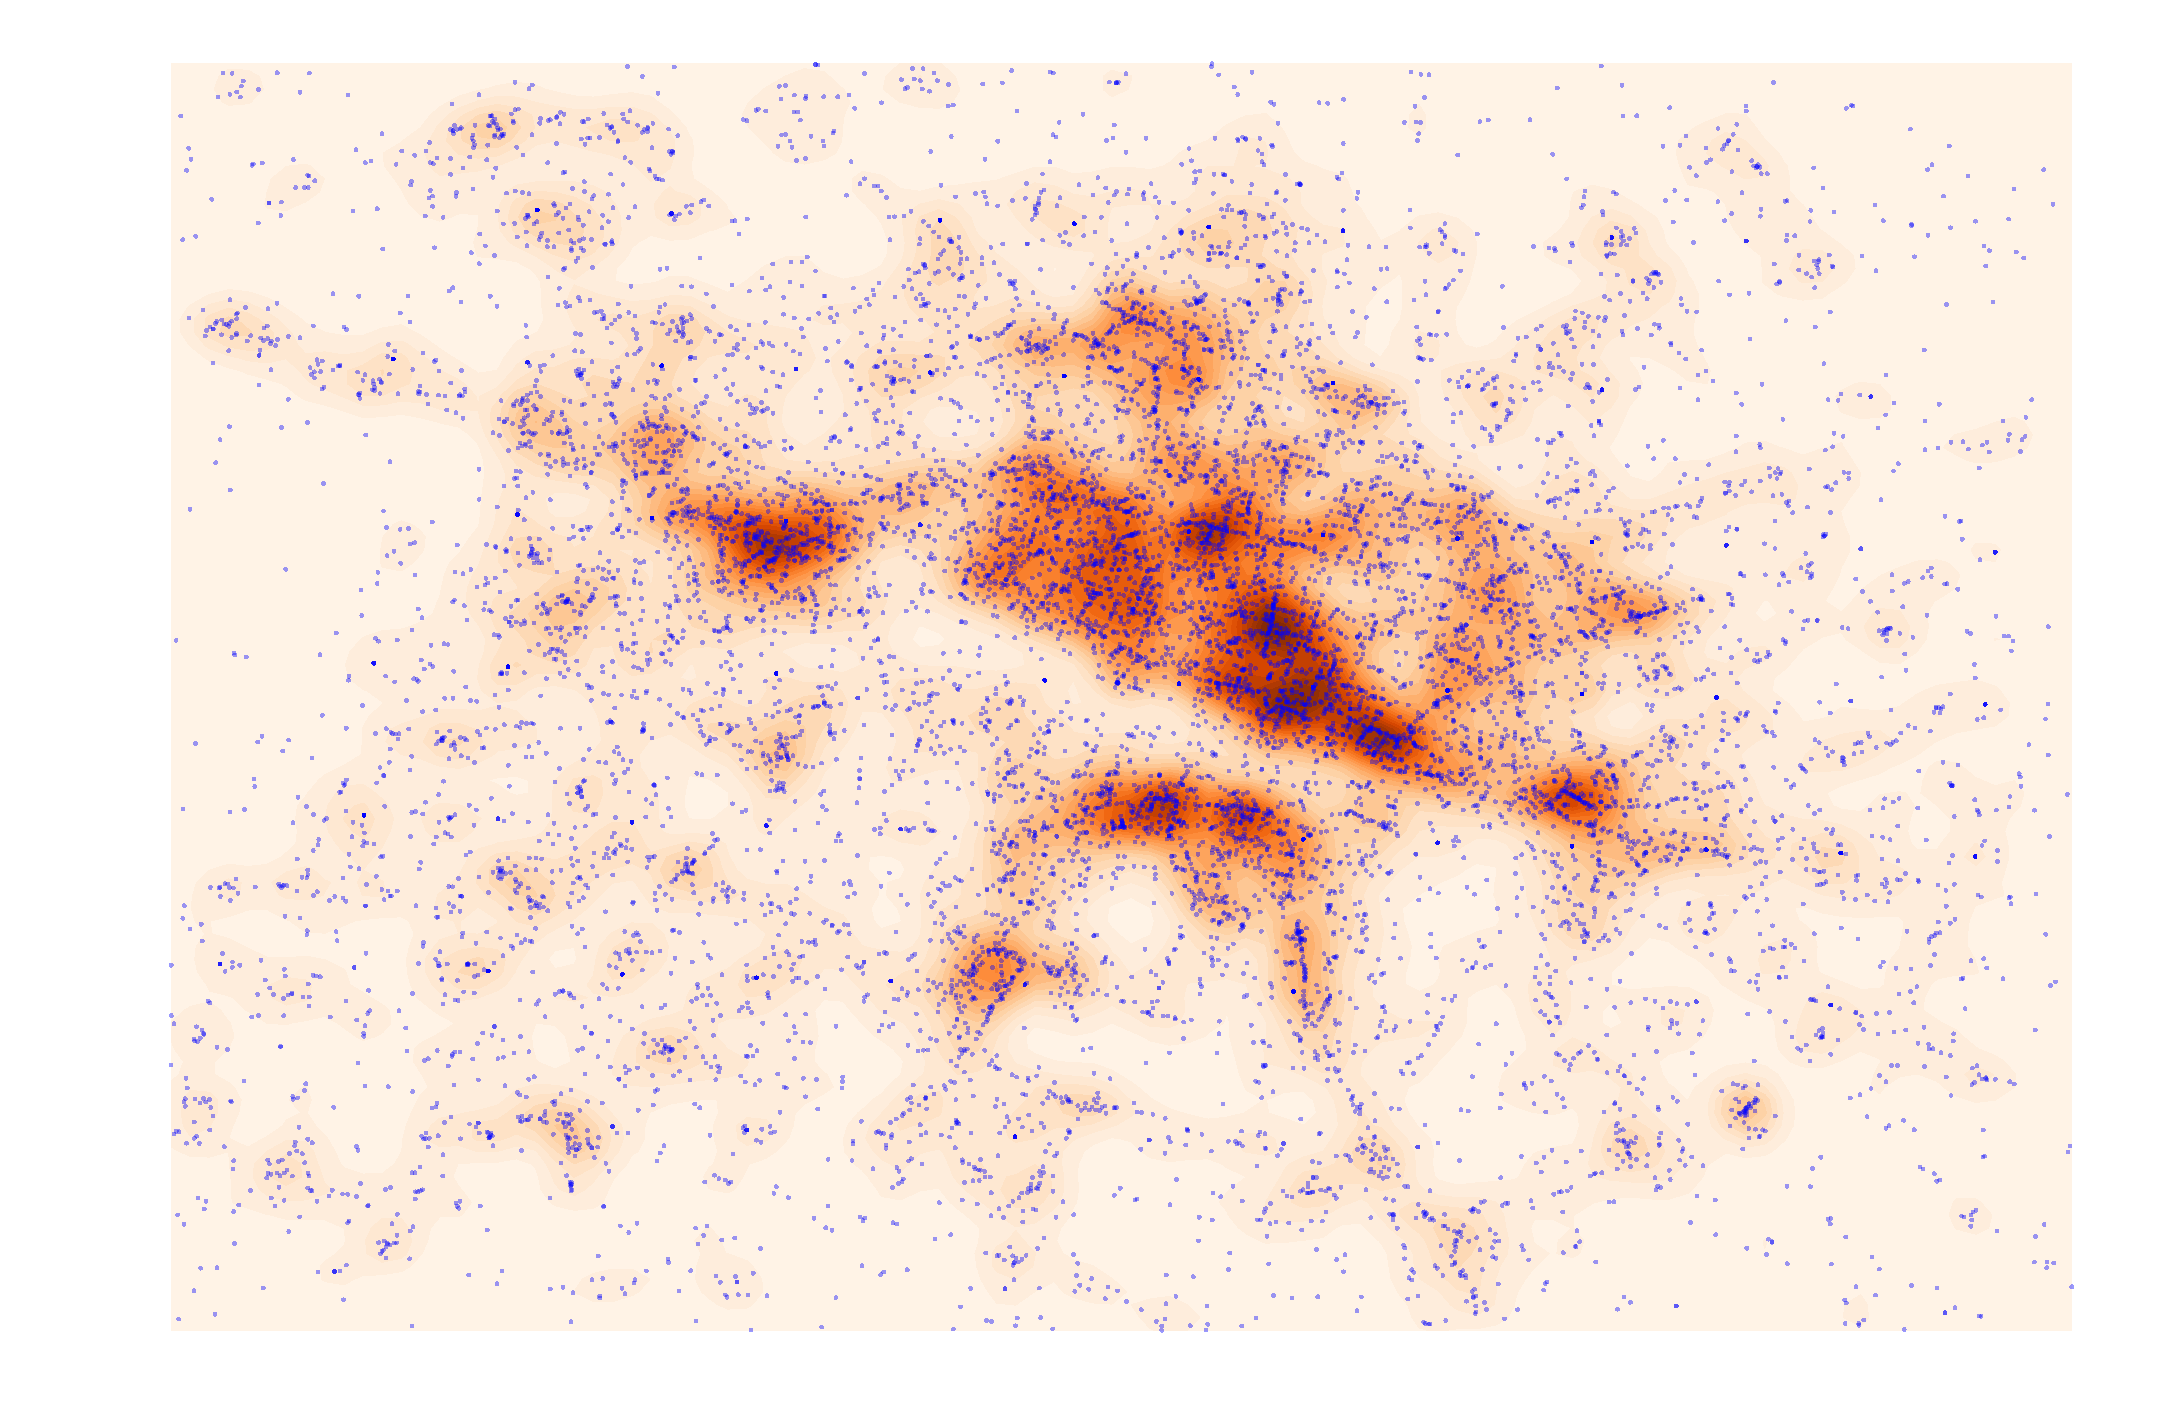
\includegraphics[width=\textwidth]{density_paris_venues}
\caption[Venue density in Paris]{Estimated venues density in Paris.
\label{fig:density_paris}}
\end{figure}

Density picture \autoref{fig:density_paris} remote versus central
locations

Explain categories surrounding.

\subsection{User entropy}

Explain why entropy is an interesting measure according to
\autocite{Entropy10}.

Let $\mathcal{U}$ be the set of users and $\mathcal{V}$ the one of venues. For
each venue $v \in \mathcal{V}$, we can gather the set of check-ins $c_v$ that
occurred there as well as the corresponding users $[u_1, u_2, u_2, \ldots,
u_n]$ (note that the same users can check-in multiple times). Then we
transform this list to a frequency distribution $f_v$ over $\mathcal{U}$ and
compute the normalized entropy: \[
    H(v) = -\frac{1}{\log\left(\left| \mathcal{U}\right|\right)}
\sum_{u\in \mathcal{U}} f_v(u) \log(f_v(u)) \]

Show example with high and low value in Paris and Barcelona:
\begin{tabular}{llr}
	\toprule
	Name                    & Category            & Entropy \\
	\midrule
	Castellers de Barcelona & Non-Profit          & 0.118064 \\
	Café de la Pompeu       & Café                & 0.146145 \\
	Ràdio 4                 & Radio Station       & 0.149995 \\
	La Comarca              & Home (private)      & 0.153078 \\
	House castellar         & Home (private)      & 0.154076 \\
	Av Tomas Gimenez        & Bar                 & 0.158411 \\
	Torre De Barad-Dur      & Building            & 0.163024 \\
	\midrule
	Parc de la Ciutadella   & Park                & 4.416021 \\
	Apple Store             & Electronics Store   & 4.560921 \\
	Parc Güell              & Park                & 4.815076 \\
	Plaça de Catalunya      & Plaza               & 4.977019 \\
	Sagrada Família         & Government Building & 5.356548 \\
	Sants Estació           & Train Station       & 5.360970 \\
	Camp Nou                & Stadium             & 5.829855 \\
	\bottomrule
\end{tabular}

Compute time entropy and see if there is a link. Not really, some place are
visited all the day by a very small group of people,
\autoref{fig:two_entropies}

\begin{figure}[hbtp]
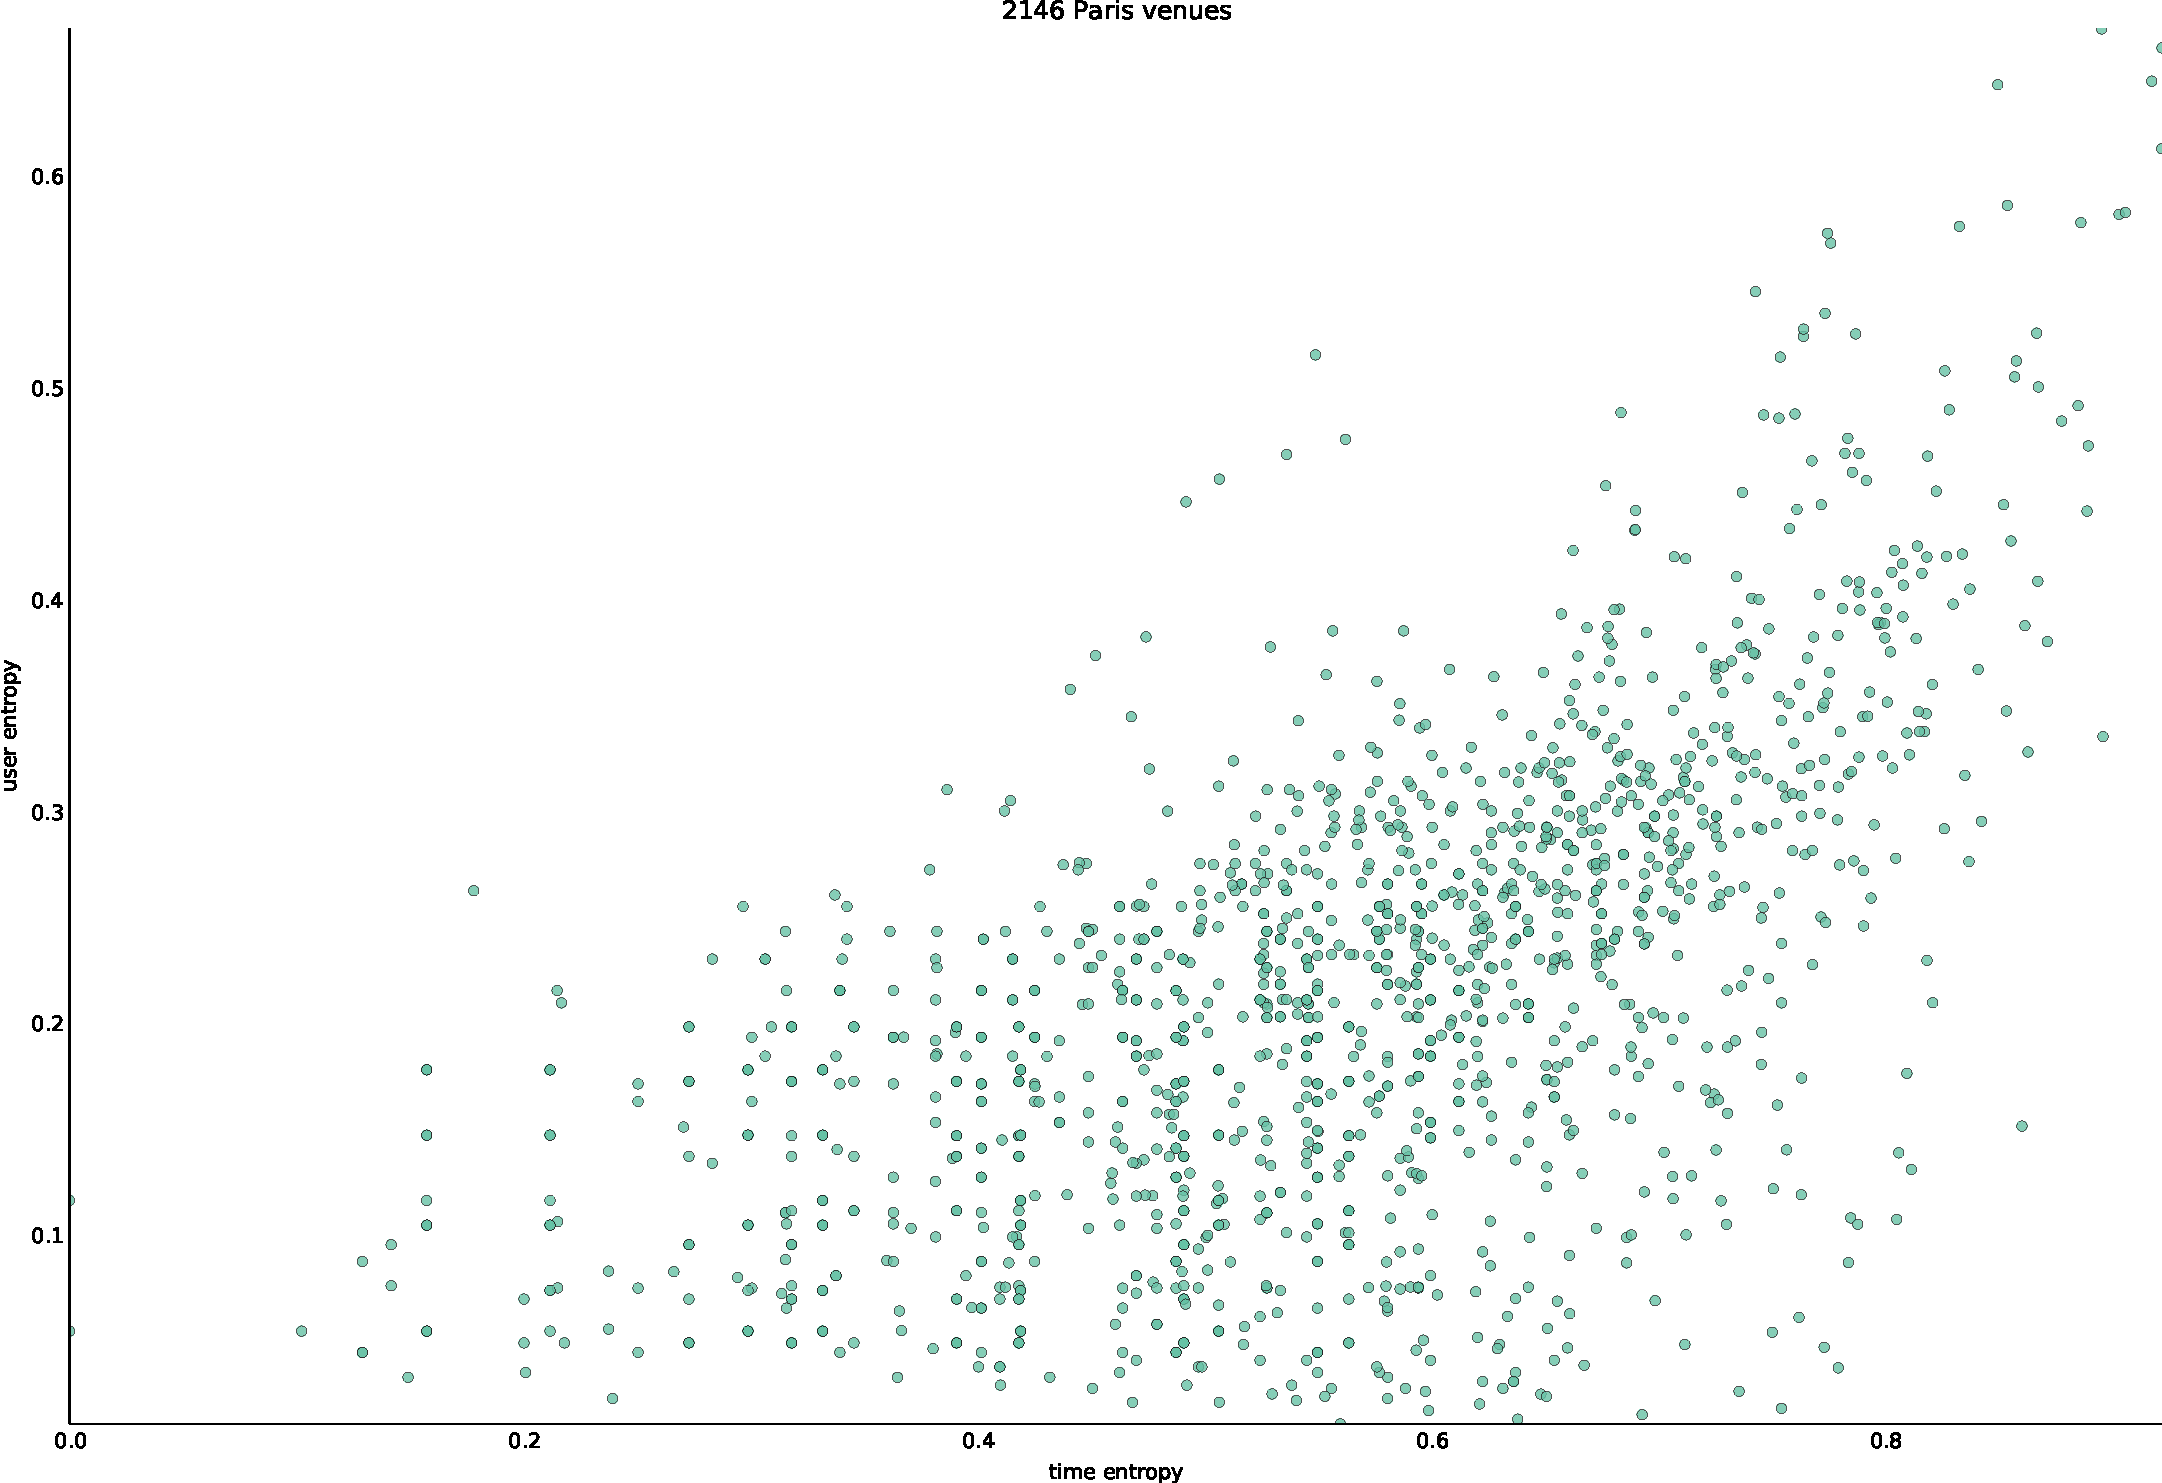
\includegraphics[width=\textwidth]{two_entropies}
\caption{Venues entropy with respect to user population and time of check-in
during the day. \label{fig:two_entropies}}
\end{figure}


\subsection{Photos}

Assume that photos are background signal of interest within city. Use exact
grid algo from \autocite{Agarwal2006spatial} to compute discrepancy with
check-ins measurement (and conversely). \marginpar{give real examples} More
photos in touristic places, more check-in in “event” places (railway, stadium)

Look at high and low focus places: not so interesting either. High value are
for popular places like park or monument whereas low (but not zero) are for
mundane place (like pizzeria) close to famous locations.

\section{Chosen representation}

Based on the insights gained by exploring the dataset, we settle to represents
each venues by the numerical vector presented in \autoref{tab:venuefeatures}.
The features involving the surrounding (numbered from 6 to 16) were weighted
by a 2D Gaussian of radius $r=350$ meters.

\begin{table}[hb]
    \centering
    \begin{tabularx}{\textwidth}{lX}
        \toprule
        index & description \\
        \midrule
	\datasetRow{}0 & Number of likes \\
	\datasetRow{}1 & Number of unique users \\
	\datasetRow{}2 & Number of total check-ins \\
        3 & User entropy \\
        4 & Venue density \\
	\datasetRow{}5 & Venue top level category \\
        6 & \enquote{Arts \& Entertainment} venues around \\
        7 & \enquote{College \& University} venues around \\
        8 & \enquote{Food} venues around \\
        9 & \enquote{Nightlife Spot} venues around \\
        10 & \enquote{Outdoors \& Recreation} venues around \\
        11 & \enquote{Shop \& Service} venues around \\
        12 & \enquote{Professional \& Other Places} venues around \\
        13 & \enquote{Residence} venues around \\
        14 & \enquote{Travel \& Transport} venues around \\
	15 & Ratio of photos over check-ins \\
	16 & Ratio of photos associated to the venue over photos linked to other venues \\
	17 & More than half of the check-ins occurs during the week-end \\
	18 & Frequency of check-ins between 2 a.m. and 6 a.m. \\
	19 & Frequency of check-ins between 6 a.m. and 10 a.m. \\
	20 & Frequency of check-ins between 10 a.m. and 2 p.m. \\
	21 & Frequency of check-ins between 2 p.m. and 6 p.m. \\
	22 & Frequency of check-ins between 6 p.m. and 10 p.m. \\
	23 & Frequency of check-ins between 10 p.m. and 2 a.m. \\
        \bottomrule
    \end{tabularx}
    \caption[Venue features]{Feature representation of Foursquare venues,
	    taking surrounding into account. \colorbox{Moccasin}{Shaded
	    features} are provided directly by Foursquare database whereas the
	    others were computed solely based on the partial information
	    contained in the dataset.\label{tab:venuefeatures}}
\end{table}

\clearpage

\newgeometry{hmargin=1.1cm,vmargin=0.7cm}
\begin{table}[t]
	\centering
	\begin{tabularx}{\textwidth}{lXX}
		\toprule
		field & description & example \\
		\midrule
		\texttt{\_id}   & Flickr photo id                                    & 12683984675 \\
		\texttt{loc}    & GeoJSON location of the photo                      & {"type": "Point", "coordinates": [25.009667, 60.227586]} \\
		\texttt{uid}    & Flickr user id                                     & "40747751@N08" \\
		\texttt{taken}  & Local time of the shooting according to the camera & ISODate("2014-02-21T18:40:21Z") \\
		\texttt{title}  & User given title                                   & "One Way to Lock a Bicycle" \\
		\texttt{hint}   & city name                                          & "helsinki" \\
		\texttt{tags}   & Normalized user given tags                         & ["bicycle", "lock", "chain", padlock, "locked"] \\
		\texttt{venue}  & Foursquare venue id                                & null \\
		\texttt{upload} & UTC time at which the photo was uploaded           & ISODate("2014-02-22T00:28:32Z") \\
		\texttt{farm}   & Used to obtain a link to the picture file          & 6 \\
		\texttt{server} & Used to obtain a link to the picture file          & "5506" \\
		\texttt{secret} & Used to obtain a link to the picture file          & "74fbd5b60a" \\
		\bottomrule
	\end{tabularx}
	\caption[Photo format]{Description of the fields of the photo
	object.\label{tab:photo}}
\end{table}
\begin{table}[b]
    \centering
    \begin{tabularx}{\textwidth}{lXX}
        \toprule
        field & description & example \\
        \midrule
\texttt{\_id}          & Foursquare venue id                             & "4ba22d4cf964a5207ce137e3" \\
\texttt{name}          & Name of the venue                               & "Ravintola Oiva" \\
\texttt{loc}           & GeoJSON location according to Foursquare        & {"type" : "Point", "coordinates": [24.951011, 60.181716084480286]} \\
\texttt{cat}           & id of the primary category                      & "4bf58dd8d48988d11b941735" \\
\texttt{cats}          & Potential additional categories                 & ["4bf58dd8d48988d1c4941735", "4bf58dd8d48988d143941735"] \\
\texttt{checkinsCount} & Total number of check-ins in Foursquare         & \numprint{2556} \\
\texttt{usersCount}    & Number of unique user in Foursquare             & \numprint{1321} \\
\texttt{tipCount}      & Number of tip left by users                     & 13 \\
\texttt{price}         & Price range, from 1 to 4                        & 2 \\
\texttt{rating}        & Rating over 10                                  & 7.82 \\
\texttt{createdAt}     & Time at which the venue was added to Foursquare & ISODate("2010-03-18T15:40:28Z") \\
\texttt{mayor}         & User id of the mayor at the time of collection  & 18123276 \\
\texttt{tags}          & User contributed tags                           & ["karaoke"] \\
\texttt{shortUrl}      & Short URL appearing in tweets                   & "\url{http://4sq.com/bV8IRQ}" \\
\texttt{canonicalUrl}  & Full URL                                        & "\url{https://foursquare.com/v/ravintola-oiva/4ba22d4cf964a5207ce137e3}" \\
\texttt{likes}         & Total number of like in Foursquare              & 3 \\
\texttt{likers}        & List of at most ten users liking this venue     & [14695530, 9936722, 37114401] \\
\texttt{city}          & City name                                       & "helsinki" \\
\texttt{closed}        & True when Foursquare says the venue is closed   & null \\
\texttt{hours}         & Always \texttt{null}                            & null \\
        \bottomrule
    \end{tabularx}
    \caption[Venue format]{Description of the fields of the venue
    object.\label{tab:venue}}
\end{table}
\restoregeometry
